\documentclass[a4paper, 11pt]{article}
\usepackage{comment} % enables the use of multi-line comments (\ifx \fi) 
\usepackage{lipsum} %This package just generates Lorem Ipsum filler text. 
\usepackage{fullpage} % changes the margin
\usepackage{graphicx}
 \usepackage{cite}
 \usepackage{appendix}
 
 \usepackage{listings}
\usepackage{color} %red, green, blue, yellow, cyan, magenta, black, white
\definecolor{mygreen}{RGB}{28,172,0} % color values Red, Green, Blue
\definecolor{mylilas}{RGB}{170,55,241}

\usepackage{csvsimple}
\usepackage{pgfplotstable}
\usepackage{booktabs}
\usepackage{amsmath}
\usepackage{adjustbox}
\usepackage{graphicx}
\usepackage{tikz}
\usetikzlibrary{shapes,positioning,matrix}
\usepackage{neuralnetwork}
\usepackage{tikz}
%\usetikzlibrary{...}
\usepackage{standalone}
\usepackage{subcaption}

\begin{document}
%Header-Make sure you update this information!!!!
\noindent


\part*{Section A}
\section*{Architecture Discussion}

\subsection*{Problem}
The problem is a two class classification problem - occupancy detection based on sensor readings. The recorded sensor data is temperature, humidity, light and carbon dioxide. The features include an additional derived feature, humidity ratio, which was derived from the original recorded variables. Each point in the data set is also timestamped. In \cite{Candanedo2016} the time stamp was used to derive two additional features - week status(WS) and number of seconds from midnight(NSM).
A certain amount of noise is expected in the recorded data so a suitable architecture should have good generalisation. Since data was measured in a controlled environment we expect the range of training variables to roughly match the range of expected data.

\subsection*{Architectures}
There are several neural network architectures suitable for this kind of classification problem - Multilayer perceptron, Radial basis function network and Correlation memory matrix. 
\subsubsection*{Multilayer Perceptron (MLP)}
MLP is a feedforward neural network with multiple neurons composed in multiple layers. All neurons are the same in the case of classification and they compute a weighted sum of inputs and apply an activation function (sigmoid or tanh). There is an input layer, which distributes the inputs, zero or more hidden layers and an output layer. Each layer feeds into the next one. This type of neural network uses and error correcting learning rule and a backpropagation training algorithm. Backpropagation consists of two stages - a forward pass, where outputs are computed and a backward pass where weights are adjusted according to the error in outputs. In the backward pass the output layer weights are adjusted according to the local gradient of the error function and the hidden layer weights are adjusted according to the local gradients of the nodes in the subsequent layer. 
\subsubsection*{MLP Advantages and disadvantages}
The multilayer perceptron is suiatable for nonlinearly seperable classification problems. Once a good aproximate solution is found generalisation can be easyly improved by adjusting the stopping criteria of the training algorithm or using regularisation. MLP is a global approximator (because it split's the entire pattern space using lines), which can be an advantage if dataset we have doesn't describe the full range of expected data. \\ 
Determining the number of hidden layers and number of neurons in each layer may require a lot of experimentation. The training algorithm uses local gradients and can often get stuck in a local minimum of the error function. 


%MLP is a feedforward, multilayer architecture consisting of one input layer, one output layer and hidden layers. The input layer just passes on the inputs. Each neuron in the hidden layers computes a weighted sum of inputs, applies a transfer function and passes it's output to each neuron in the next layer. Each layer feeds into the next and the output layer produces the outputs. The MLP uses an error correction learning rule, where it minimises an error function defined by the difference of it's output and the desired output (typically the error function is mean squared error). In order to minimise the error function, it needs to be continuous, therefore the transfer function of each neuron is either a hyperbolic tangent function or a sigmoid function. The training algorithm for MLP is backpropagation. It consists of a forward pass, where the network computes it's output and a backward pass, where the weights are adjusted. Weight changes at each layer are computed based on the local gradient of the next layer. The MLP classifies patterns by partitioning the feature space into regions. It can be used to solve linearly inseparable classification problems, as each layer computes a non-linear transformation of the outputs of the previouse one.
\subsubsection*{Radial Basis Function Network (RBF)}
RBF is a feedforward network, consisting of single hidden layer and an input and output layer. Input layer just distributes inputs to the hidden layer. Each neuron in the hidden layer computes a radially symmetric basis activation function (typically a Gaussian) from the inputs. The output layer neurons compute a weighted sum of the outputs of the hidden layer. Each neuron in the hidden layer has two associated parameters - a point in the feature space, which is called a center, and a spread. It computes it's response to a given input based on the euclidean distance between the data point and it's center. Training is typically done in two stages - center selection and weight estimation, where wighgts can be cimputed in a single matrix vector calculation. RBFs can also be trained in a supervised manner (like MLP) or by selecting centers at each data point and using regularisation, but these aproaches are much slower.
\subsubsection*{RBF Advantages and Disadvantages}
There is only one hidden layer so we only need to experiment with it's size. When using unsupervised center selection, weights can be computed in a single calculation. There are much less architecture parameters that can be varied when searching for an  architecture compared to the MLP. The RBF is a local approximator, which is an advantage when we expect new data to be in a similar range to the training data or when abnormal inputs need to be ignored. \\
It is difficult to determine center locations. When data isn't clustered might need a very large hidden layer.  Supervised center selection and regularisation training approaches are very slow. 

\subsubsection*{Correlation Matrix Memory(CMM)}
CMMs are single layer neural networks, which use the Hebbian learning rule. They consist of a single weight matrix which stores correlations between input and output patterns. Learning is done by computing the outer product of the input and output and adding it to the outer products of all other patterns to form the weight matrix. Recall of a stored pattern is done by multiplying the weight matrix and the input. For efficiency these networks usually have binary inputs and weights. In order to use a CMM as a classifier the output needs to be threasholded, so the highest output value is set to 1 and represents the class, or some kind of postprocessing needs to be done such as the one used in \cite{Zhou1998}.  
\subsubsection*{CMM advantages and disadvantages}
A hardware implementation of CMM can be very fast. Training and recall are both very fast operations. \\
A CMM can store a limited number of pattern associations after which new associations become diluted. Real valued data needs to be encoded using a binning algorithm. Best performance requires input patterns to follow a uniform distribution. Good classification might require additional post processing (e.g. k nearest neighbours).

%\subsubsection*{Advantages/Disadvantages}
%The Perceptron is a very simple and quick to train network consisting of a single neuron. However it can easily be ruled out because of it's inability to classify linearly inseperable problems. From figure \ref{fig:plotmatrix} we can clearly see that our data is linearly inseperable when looking at the relation between Hummidity and CO2 for example. 
%The MLP is suatable for solving non-linearly seperable problems. It's iterative training process can be slow depending on the error function minimisation method used, however it is very customisable. Once a good aproximate solution is found generalisation can be easyly improved by adjusting the stopping criteria of the training or employing regularisation. Choosing the right size of the network might require a lot of trial and error. The MLP is global aproximator, which might be an advantage when we could expect new data to be significantly different from training data.
%The RBF has a single hidden layer. Training can be very slow when using supervised selection of centers or regularisation. There are much less architecture parameters that can be varied when searching for a suitable architecture compared to the MLP. The RBF is a local aproximator, which is an advantage when we expect new data to be in a similar range to the training data and can also be used for detecting abnormal inputs. 

%\subsection*{Data exploration}
%All features - Temperature, Humidity, Light, CO2, Humidity Ratio are real valued. In figure \ref{fig:plotmatrix} the MATLAB $gplotmatrix$ function is used to plot all variables against each other and create histograms of each variable along the diagonal and class are color coded.  

\subsubsection*{Choice of network architecture}
Comparing the three architectures stated above we choose an RBF network architecture. Compared to the MLP the RBF has a simpler training process. Furthermore, using our knowledge of the problem we can see that the data we have should more or less be like the expected data after training. Because of this an RBF would be more suitable as a local classifier rather than an MLP.
The CMM is superior in terms of speed, and would be a very suitable choice for a real time application. However it would require further domain knowledge of the data in order to decide on encoding of inputs. The CMM's capacity limitations might mean we would need a very large weight matrix. 

\section*{Creation and Application}
The neural network architecture we are going to use is an RBF network with unsupervised center selection. As a benchmark we will use a fixed number of centres determined by the rule of thumb $m = \sqrt[3]{N}, N = number of data points$ and a spread $dmax = maximum distance between centers$ The network is implemented and tested in Matlab and the code is available in the appendix. 

\subsection*{Data}
%• Data [10 marks]
%Describe (briefly) the data you have, and how much there is of it.
%Describe the inputs to (and outputs from) the network. You need to
%describe how the data you started with have been preprocessed. Explain
%how you investigated the data, including any assumptions you have
%made. Again, this may include some testing of networks to see what the
%effects are of different preprocessing choices. Give a step by step process
%for transforming the data into the network inputs, sufficient for someone
%else to process a new batch of data for use with the trained network. If
%you have transformed inputs using PCA, give the transformation matrix
%as an appendix to the report.
Three data sets are provided for training, validation and testing. The test sets are merged together according to the chronological order of the timestamps. The composite test set has 20,560 data points The timestamps themselves are not used as features. The features are Temperature, Humidity, Light, CO2, Humidity Ratio and are all real valued. The target outputs are binary. Hummidity Ratio has not been measured, it has been derived from Humidity measurements \cite{Candanedo2016}. 

In figure \ref{fig:plotmatrix} the MATLAB $gplotmatrix$ function is used to plot all input variables against each other and create histograms of each variable along the diagonal and classes are color coded. We can make several observations based on this plot. The plots of light against all other features show a clear separation of the two classes, so light is probably an important feature. On the other hand the histogram of light is bimodal and clearly the examples around the second peak are much less than around the first, which means they are under-represented and might not be properly incorporated in the model. Looking at CO2 we see that it's distribution is skewed, which also might cause problems for our model. The other distributions of variables look normal. 

\begin{figure}[h]
  \caption{Plot matrix}
  \centering
    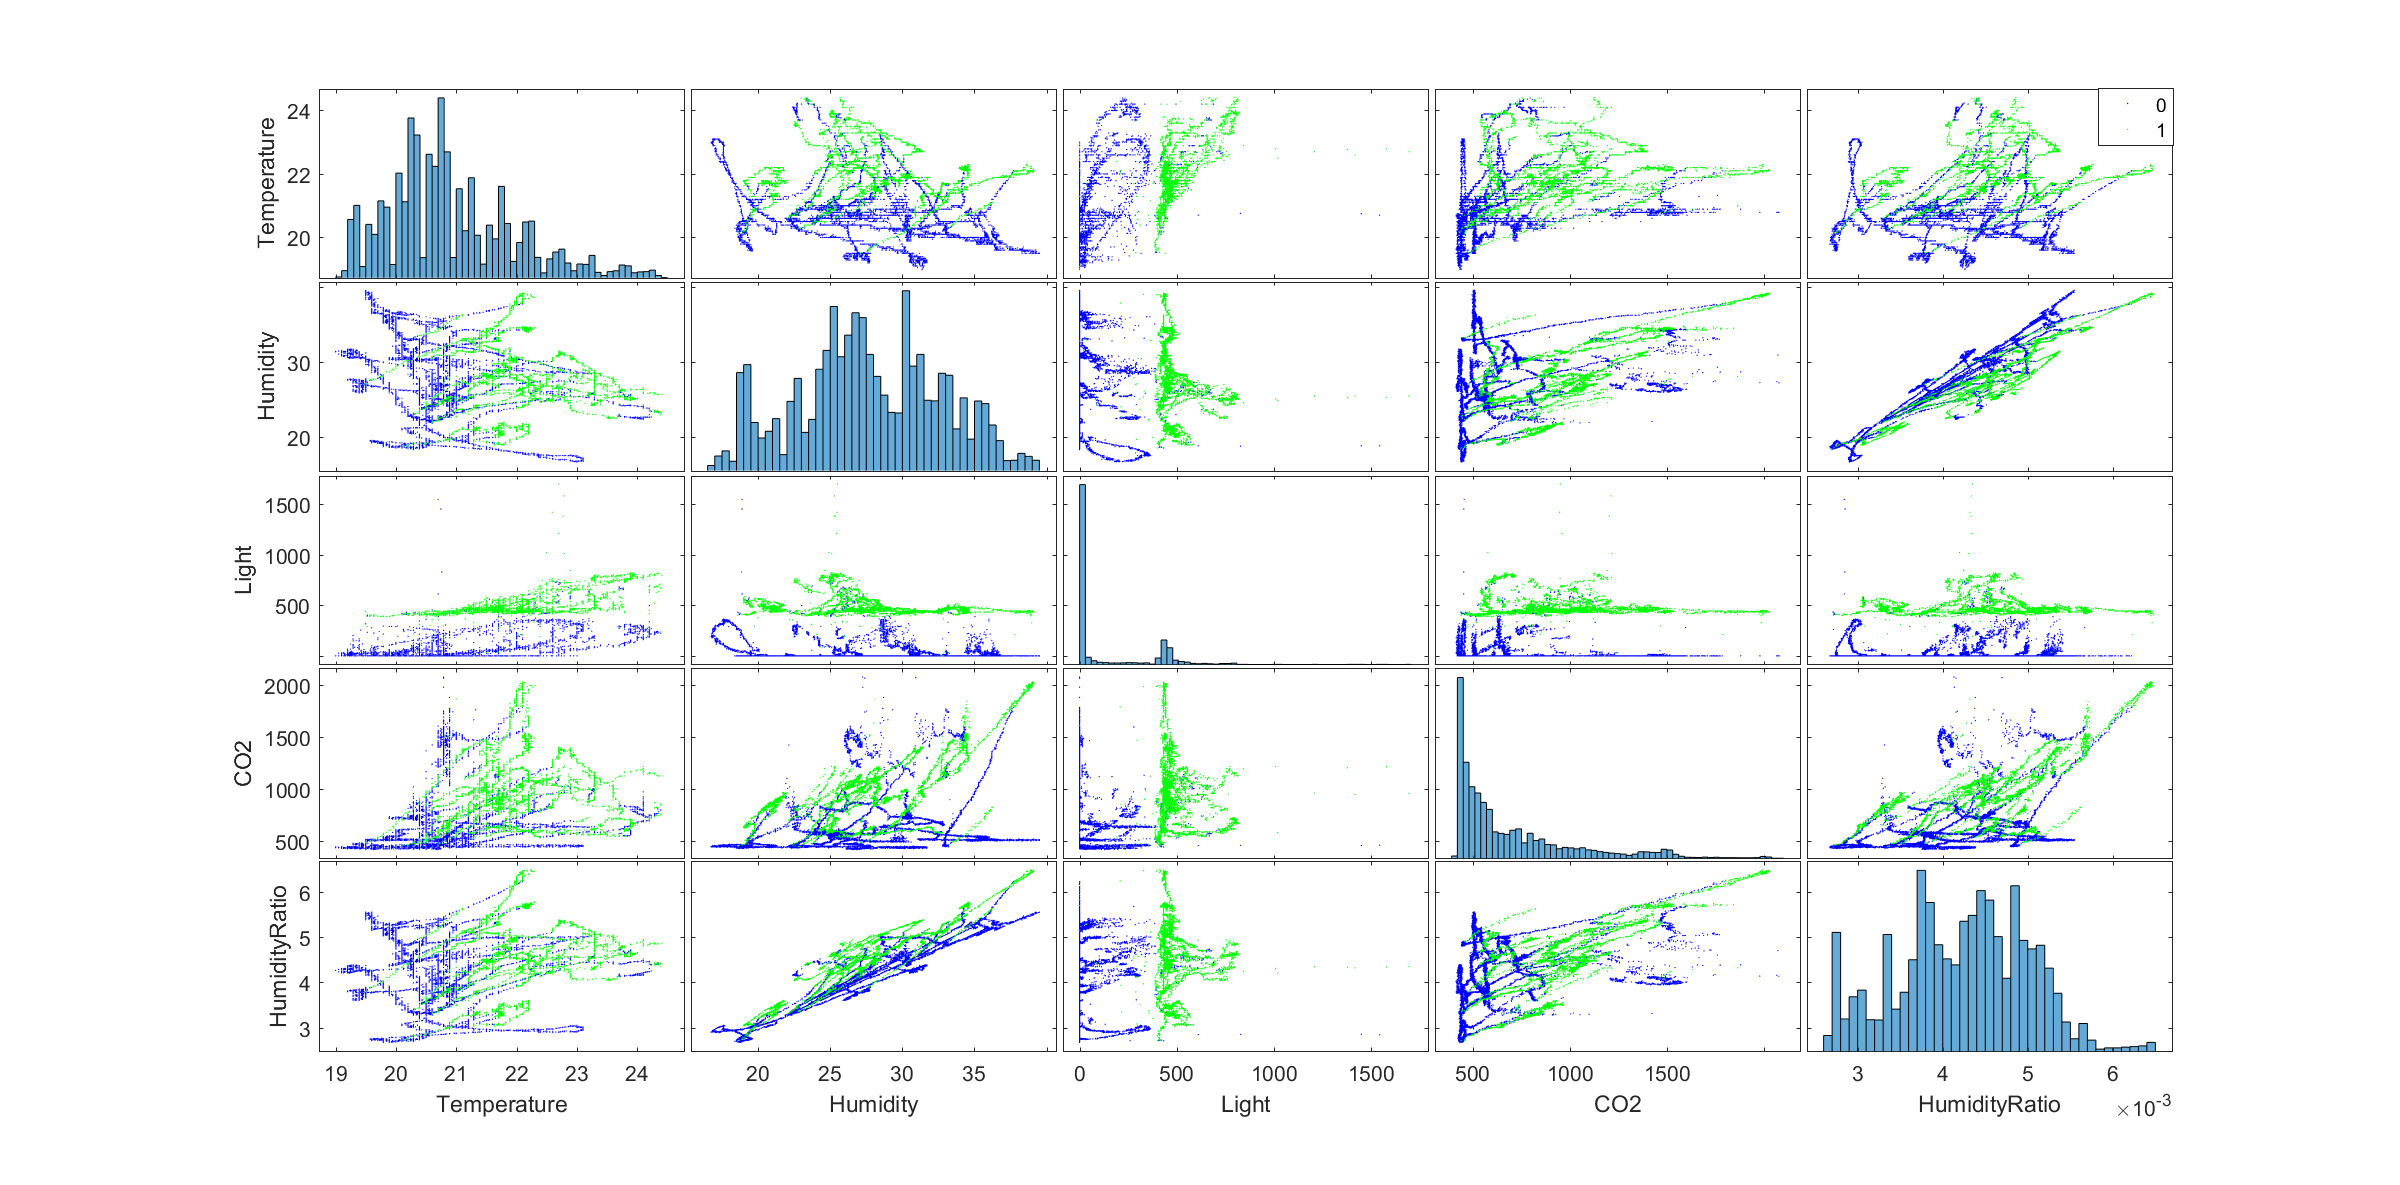
\includegraphics[width=1\textwidth]{../figures/plotmatrix.png}
    \label{fig:plotmatrix}
\end{figure}

There seems to be a big correlation between Hummidity and HummidityRatio, which makes sense since the later is derived from the first one. It might be a good idea to discard HummidityRatio. However to make sure that we are really removing unimportant features and be able to measure their contribution to the dataset we use Principal component analysis (PCA). PCA does two things. It orthogonalises input components to remove correlation between them. It can also be used to remove principal components which have very little contribution towards the total variance of the data. Since PCA is sensitive to big variances in the data we first preprocess the data to have a variance of 1 (using Matlab $mapstd$ function) and then we apply PCA (Matlab $pca$ function). PCA gives us the eigenvectors and eigenvalues of the covariance matrix of the data. The eigenvectors are the transformed inputs (prinicpal components) and the eigenvalues tell us how much each component contributes to the overall variance. Looking at figure \ref{fig:eigenvalues} we can see that the eigenvalue for the fifth principal component is only 0.001 and in terms of percentage, the contribution of this component to overall variance is 0.03\%. This means that the fifth principal component hardly has any contribution on the variance of the data. Removing it wouldn't affect the separability of the data but might make network training more efficient. The forth principal component has a much greater contribution to overall variance (6.3\%) so we decide keep it. The threashhold for eigenvalues of principal components has to be between the value of the forth and fifth. We decide to set it at 0.02. 

\begin{figure}[h]
  \caption{Eigenvalues and percent contribution to overall variance of each principal components}
  \centering
    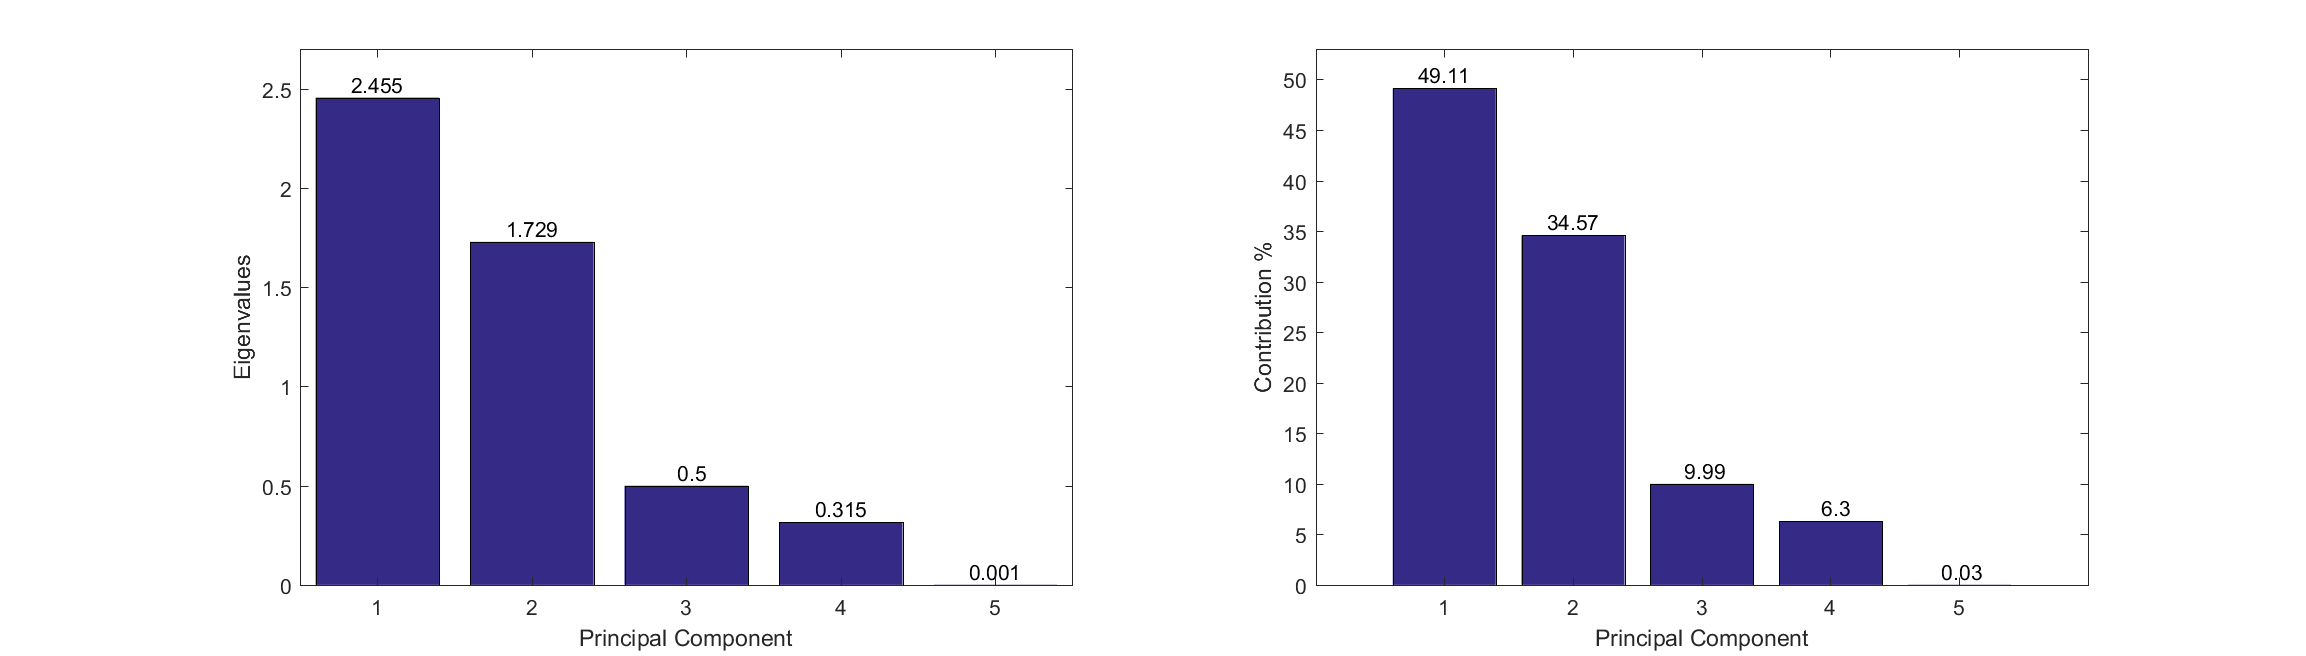
\includegraphics[width=1\textwidth]{../figures/eigenvalues.png}
    \label{fig:eigenvalues}
\end{figure}

Furthermore, looking at figure \ref{fig:pca_plotmatrix} we see that the distributions of all 4 principal components are more or less normal, which means we don't have to worry about potential problems arising from the skewed CO2 distribution or asymetric bimodal distribution of Light. 

\begin{figure}[h]
  \caption{Plot matrix of principal components}
  \centering
    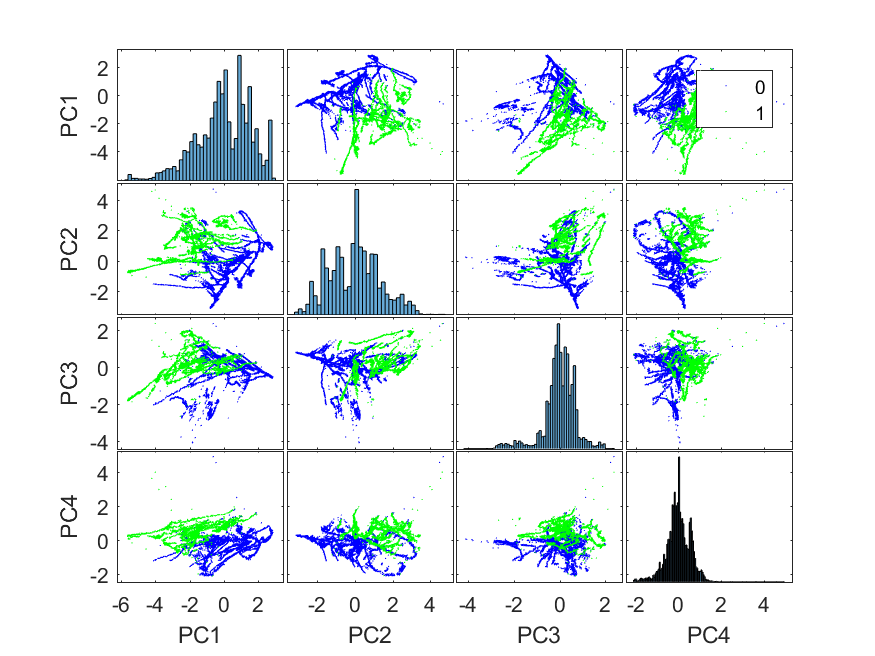
\includegraphics[width=0.5\textwidth]{../figures/pca_plotmatrix.png}
    \label{fig:pca_plotmatrix}
\end{figure}

In the end, preprocessing of the input data consist of normalising variances of features to 1. And applying a transformation using principal component analysis, removing principal components with eigenvalues less than 0.02. We use the Matlab functions $x1, trans1 = mapstd(x)$ and $x2, trans2 = processpca(x1, 0.02)$. The transformation settings $trans1$ and $trans2$ are provided in the appendix in table \ref{table:mapstd} and table \ref{table:pca}.
  











\subsection*{Network}
\begin{figure}[h]
\centering
  \includestandalone[width=0.5\textwidth]{diagram}%     without .tex extension
  % or use \input{mytikz}
  \caption{RBFN architecture diagram.}
  \label{fig:architecture}
\end{figure}

%You should describe the network architecture that you have found to
%be the best for solving the problem. The description of the structure of the architecture should be sufficient for someone else to implement your
%network exactly, and not necessarily using MATLAB, so you should
%include all the structural information and parameters necessary. Include
%a diagram.
%You should also indicate how you implemented it. This could be brief if
%you have used MATLAB defaults, for example.
\subsubsection*{Inputs}
Inputs are preprocessed before they are presented to the network. The data set is then randomly split into a training set and a test set with ratio 75\%/25\%.

\subsubsection*{Input Layer}
The input layer distributes inputs, after preprocessing, to each neuron in the hidden layer. The size of the input layer is therefore the size of the input vector $N=4$ (after PCA). It is fully connected to the hidden layer.

\subsubsection*{Hidden Layer}
There is a single hidden layer fully connected to the output layer. The optimal size of the hidden layer found by experimentation is $M=20$. The activation function of each neuron is an isotropic Gaussian:

\begin{equation}
\Phi_i(\boldsymbol{x}) = \exp\left(-\frac{1}{2\sigma^2} \lvert\lvert \boldsymbol{x} -  \boldsymbol{c_i} \rvert\rvert ^2\right)
\quad \mathrm{where }\quad
\sigma^2 = \frac{1}{2}(\epsilon \times d_{max})^2
\label{eq:rbf}
\end{equation}

Where $m$ is the number of hidden neurons (number of centres), $d_{max}$ is the maximum distance between centres, $\epsilon$ is a parameter used to vary the spread of the Gaussian ($0<\epsilon<2$) and $\boldsymbol{c_i}$ is the center vector of neuron $i$. The centres for each hidden layer neuron are found using a k-means clustering algorithm. The number of centres $\boldsymbol(c_i)$ and spread parameter $\epsilon$ were found through experimentation.

\subsubsection*{Output Layer}
The output layer calculates a weighted sum of hidden layer outputs:

\begin{equation}
y(\boldsymbol{x}) = \displaystyle\sum_{i=1}^{m} w_i \Phi_i(\boldsymbol{x})
\end{equation}

In order to obtain hard classification output a threshold is applied to $y(\boldsymbol{x})$ - if $y>0.5$ output is 1, else output is 0. The outputs use a boolean encoding, where 1 signifies occupancy.

\subsubsection*{Best found architecture}
The best architecture found through experimentation uses k-means algorithm to find center locations. The experimentally discovered parameter values are $m = 20, \epsilon = 0.8$. The network architecture and parameters are given below in table \ref{table:architecture}.

\begin{table}[h!]
\centering
\begin{tabular}{|l l|} 
 \hline
 Network type & Radial basis function network  \\ 
 \hline
 Data features/inputs & Temperature, Humidity, Light, CO2, HumidityRatio\\
 Data preprocessing & Normalize standard deviation to 1 \\
 & Principal component analysis (PCA) \\
 PCA variance threshold & 0.02 \\ 
 Data train/test set split & Random 75\%/25\% \\
 \hline
 Hidden layer activation function (RBF) & $
\Phi_i(\boldsymbol{x}) = \exp\left(-\frac{1}{(\epsilon \times d_{max})^2} \lvert\lvert \boldsymbol{x} -  \boldsymbol{c_i} \rvert\rvert ^2\right)  
$  \\
 Hidden layer size ($m$) & 20  \\
 RBF spread $\sigma^2$ & $\frac{1}{2}(0.8 \times d_{max})^2$   \\
 \hline
 Output layer activation function & Linear: $y(\boldsymbol{x}) = \displaystyle\sum_{i=1}^{m} w_i \Phi_i(\boldsymbol{x})$ \\
 Output layer size & 1 \\
 \hline
 Training algorithm & 1. Unsupervised center selection \\ 
 & 2. One step weight calculation using matrix pseudo inverse  \\
 Centre selection algorithm & k-means clustering \\
 Backprop performance function & Mean Squared Error (MSE)  \\ [1ex] 
 \hline
\end{tabular}
\caption{Best found RBFN architecture.}
\label{table:architecture}
\end{table}

\subsubsection*{Implementation}
The RBF network was implemented in Matlab following the solution from practical session. The code is given in the appendix (RBFN.m). For performing experiments an additional script was used it is also provided in the appendix (runRBFN.m)


\subsection*{Training}
%Explain how you selected the best training algorithm for this problem.
%This could include testing different networks and training algorithms to
%see what might work well.
%For the training algorithm you used with the final version of the network,
%give sufficient detail for someone to implement the training algorithm.
%This does NOT mean (for example) describe gradient descent in great
%detail. It DOES mean give any parameters, initialisation, etc, even if
%they are the toolbox defaults.
Three types of RBFN training algorithms were considered - regularisation with number of hidden neurons equal to the number of data points, supervised center selection and unsupervised center selection. Unsupervised center selection was chosen out of the three because of it's performance in terms of speed. This is a two step training algorithm. The first step is selecting the center points for each hidden neuron. The second step is  calculating the output layer weights based on the outputs of the hidden layer in order to minimise an error function (MSE in this case). After having selected the center points and preprocessed the data, the training algorithms goes through the following steps, assuming center points are in a matrix $c$, preprocessed training data is in a matrix $x$, the target data is stored in a binary vector $D$ and the predefined number of centres is $m$:
\begin{list}{•}{•}


\item[1] Calculate the euclidean distance from each of the centres (columns of $c$) to each of the data points (columns in $x$) and store them in a matrix $distance$. Calculate the distances from centres to centres and store them in a matrix $dc$.  
\item[2] Find the maximum center to center distance and store it in $d_{max}$. $d_{max}$ is then used to calculate the spread of all radial basis functions in the hidden layer: $\sigma^2 = \frac{1}{2}(\epsilon \times d_{max})^2$, where $\epsilon$ is a user defined parameter. 
\item[3] Calculate a matrix of responses from each basis function to each data point. Using equation \ref{eq:rbf} this calculation would be:
\begin{equation}
F = \Phi_i(\boldsymbol{x}) = \exp\left(-\frac{m}{(\epsilon \times d_{max})^2} distances^2 \right)  
\end{equation}
\item[4] Calculate the weights of the output layer $W$ using the pseudo inverse of $F^+$ and the target data $D$: $W= F^+D$.
\end{list}

For the center selection step of the training algorithm two options were considered - random center selection and k-means clustering. The kmeans function from Matlab was used for the second approach, which uses k-means++ algorithm \cite{Arthur2007} for generating initial center locations and then runs the k-means clustering algorithm \cite{Lloyd82} to iteratively search for the true center locations. In order to decide which one to use an experiment was performed using two networks, structurally the same as the one in table \ref{table:architecture},but with number of centres $m = 10, 15, 20, 25$ and $\epsilon = 1$. The two networks use the two different center selection algorithms. They were ran 10 times for each number of centres. The results are given below in table \ref{table:centermse}

\begin{table}[h]
\centering
\begin{tabular}{| l | l | l | l | l | l |}
\hline
Number of centres (m) & 10 & 15 & 20 & 25 \\
\hline
Random center selection Test MSE mean & 0.0735 & 0.0785 & 0.0832 & 0.0649 \\
\hline
Random center selection Test MSE Std & 0.0306 & 0.0523 & 0.0499 & 0.0304 \\
\hline
K-means Test MSE mean & 0.0331 & 0.0237 & 0.0190 & 0.0187 \\
\hline
K-means Test MSE Std & 0.0032 & 0.0044 & 0.0043 & 0.0041 \\
\hline
\end{tabular}
\caption{Performance results for random centre selection and k-means}
\label{table:centermse}
\end{table}

Clearly the performance (in terms of MSE) of k-means is much better than random center selection. So this is the algorithm we will use.

\subsection*{Evaluation}
%In selecting the final network you will have to make choices about, for
%example, the number of neurons or the number of layers to use.
%– Explain what metric or metrics you used for comparison between
%networks.
%– Explain the process you went through in making the selection of
%the final architecture. If you evaluated a number of networks, give
%details of what their structures were and how they performed. You
%may summarise repeated tests of the same structure, but remember
%to give mean and variance of summary statistics.
%– Explain how you used the data in this selection process. For example,
%was it split into training, validation and test sets? How big were
%they?
We have made decisions about the network structure, training algorithm, data preprocessing and splitting into training and test sets. The parameters that need to be discovered experimentally are the number of centres (size of hidden layer) and basis function spread parameter $\epsilon$, which we introduced in the Network section.
\subsubsection*{Metrics}
MSE was used as a metric of performance. However MSE on it's own is not sufficient, because it will keep decreasing as we increase the number of nodes in the network, but if we add two many nodes the generalisation of the network will be poor. This is why in addition to MSE, we also look at the percentage of errors in each of the two classes. Ideally we want our model to make an approximately equal amount of errors in both classes. If the model develops a bias against a particular class this means that we are probably over fitting the data or not capturing the structure of the data.



\subsubsection*{Experimentation for determining final network}
Initially we consider only the number of centres $m$ and search for networks with low MSE and approximately equal percentage of errors in both classes. We set the spread parameter of the network $\epsilon = 1$ and run for different hidden layer sizes $m = 5, 10, 15, 20, 25, 30, 40, 50, 60$. For each value of $m$ we train and evaluate the network 10 times and record the mean value of MSE, mean percentage of errors and mean absolute difference of errors for both the training and test sets. Results are plotted in figure \ref{fig:animals}.

\begin{figure}[h]
    \centering
    \begin{subfigure}[t]{0.32\textwidth}
        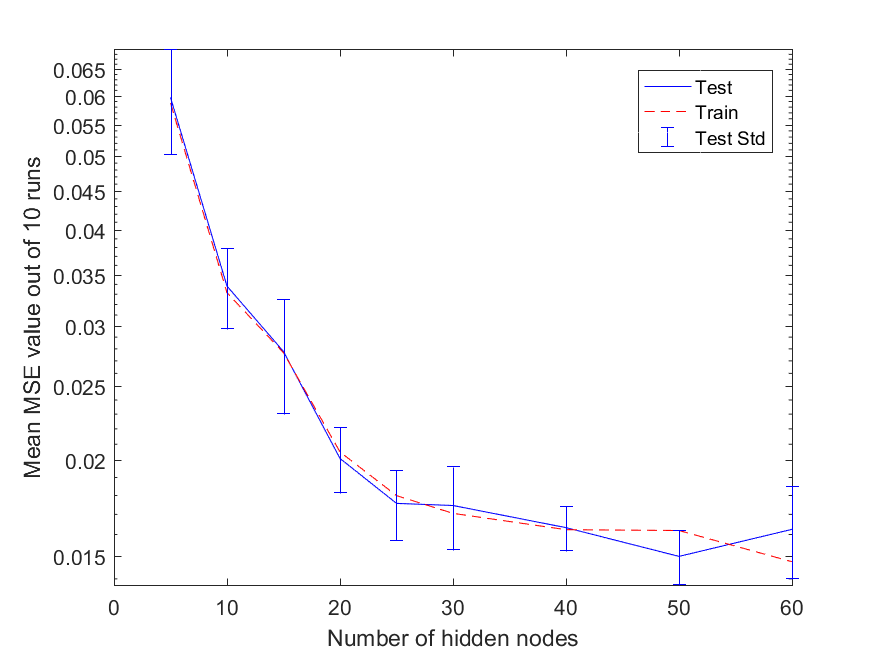
\includegraphics[width=\textwidth]{../figures/perf/mseplot_m(5-60)_e(10-10).png}
        \caption{Mean MSE of Test and Train sets.}
        \label{fig:mse}
    \end{subfigure}
    \hfill %add desired spacing between images, e. g. ~, \quad, \qquad, \hfill etc. 
      %(or a blank line to force the subfigure onto a new line)
    \begin{subfigure}[t]{0.32\textwidth}
        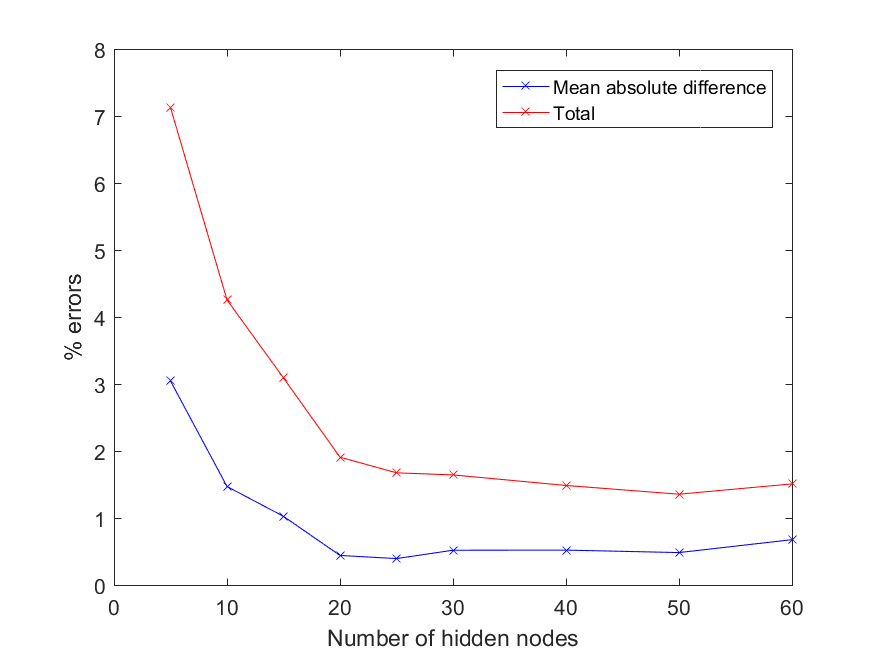
\includegraphics[width=\textwidth]{../figures/perf/errorplot_m(5-60)_e(10-10).png}
        \caption{Mean absolute difference of errors in class 0 and class 1 and mean percentage of errors in both classes, measured on test set.}
        \label{fig:errorplot}
    \end{subfigure}
    \hfill %add desired spacing between images, e. g. ~, \quad, \qquad, \hfill etc. 
    %(or a blank line to force the subfigure onto a new line)
    \begin{subfigure}[t]{0.32\textwidth}
        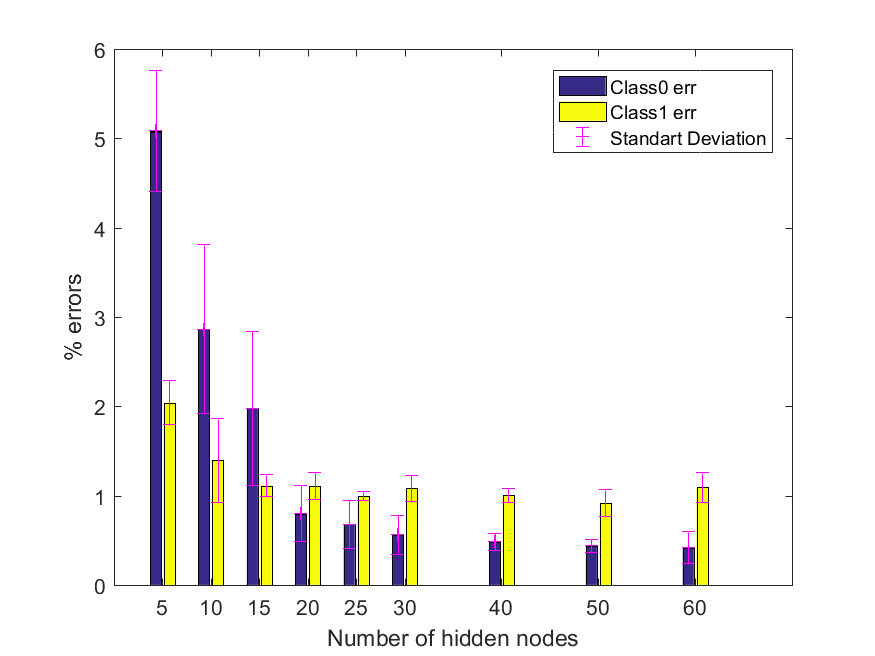
\includegraphics[width=\textwidth]{../figures/perf/errorbar_m(5-60)_e(10-10).png}
        \caption{Bar plot of mean percentage of errors in class 0 and class 1 measured on test set.}
        \label{fig:errorbar}
    \end{subfigure}
    \caption{Performance of RBFN with parameters $m = 5,15,20,25,30,40,50,60$ and $\epsilon = 1$, ran 10  times for each parameter combination.}\label{fig:performance}
\end{figure}

From figure \ref{fig:mse} above we can see that the MSE decreases when increasing the number of nodes, as we expected. After 20 hidden nodes MSE decreases at a slower rate. Looking at figure \ref{fig:errorplot} we see that after around 20 hidden nodes the mean absolute difference in errors doesn't change very much and the total number of errors decreases very slowly. These two plots give us an understanding of how performance increases by increasing number of neurons, but tells us little about how much we are overfitting the data. Looking at figure \ref{fig:errorbar} we can see that after 25 hidden nodes the errors in class 1 remain the same, while the errors in class 0 decrease. After that point the network is developing a bias against class 0. This is a hint that we are overfitting after this point. On the other hand, when we use fewer than 20 nodes the bias of the network is against the other class. This probably means we don't have enough neurons to capture the structure of the data. So we decide to use 20 hidden nodes the hidden layer and perform experiments to determine the spread coefficient $\epsilon$, while keeping $m = 20$. The results are shown in figure \ref{fig:performance1}.

\begin{figure}[h]
    \centering
    \begin{subfigure}[t]{0.32\textwidth}
        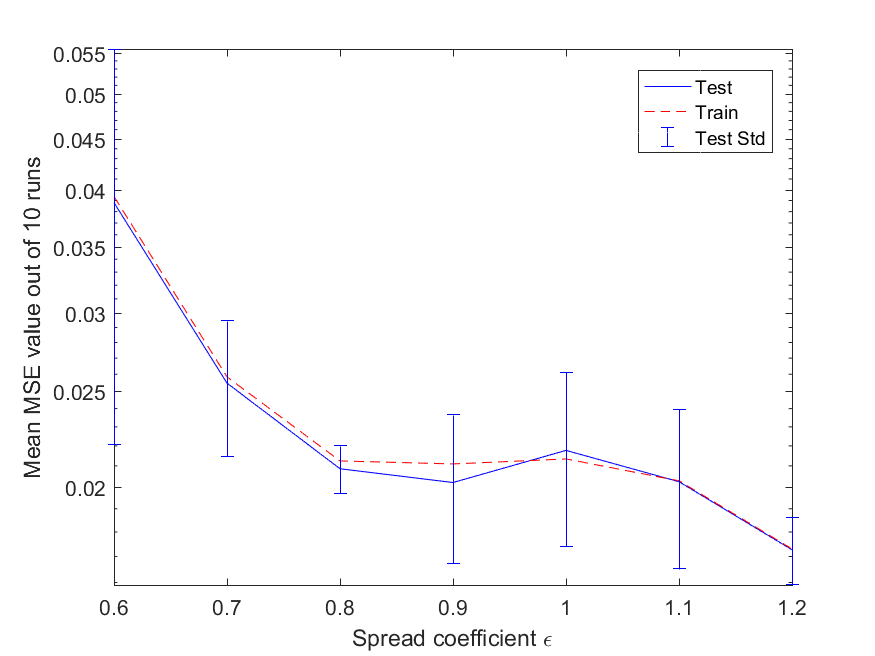
\includegraphics[width=\textwidth]{../figures/perf/mseplot_m(20-20)_e(6-12).png}
        \caption{Mean MSE of Test and Train sets.}
        \label{fig:mse1}
    \end{subfigure}
    \hfill %add desired spacing between images, e. g. ~, \quad, \qquad, \hfill etc. 
      %(or a blank line to force the subfigure onto a new line)
    \begin{subfigure}[t]{0.32\textwidth}
        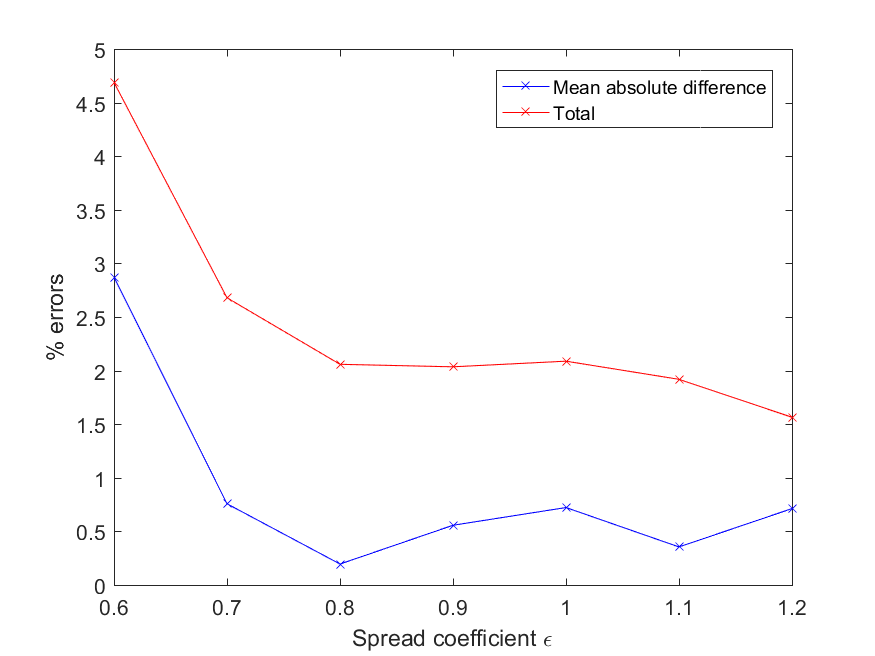
\includegraphics[width=\textwidth]{../figures/perf/errorplot_m(20-20)_e(6-12).png}
        \caption{Mean absolute difference of errors in class 0 and class 1 and mean percentage of errors in both classes, measured on test set.}
        \label{fig:errorplot1}
    \end{subfigure}
    \hfill %add desired spacing between images, e. g. ~, \quad, \qquad, \hfill etc. 
    %(or a blank line to force the subfigure onto a new line)
    \begin{subfigure}[t]{0.32\textwidth}
        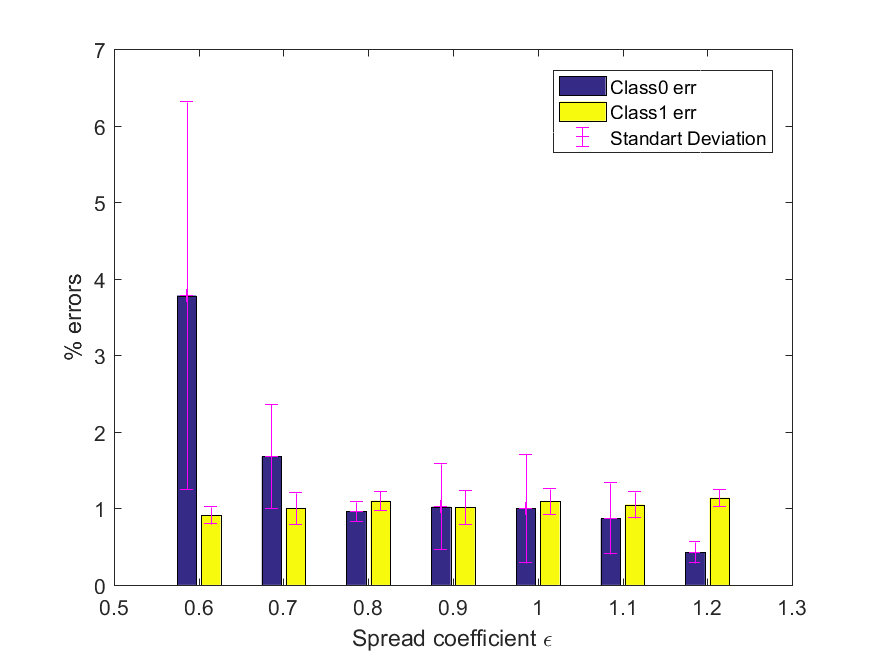
\includegraphics[width=\textwidth]{../figures/perf/errorbar_m(20-20)_e(6-12).png}
        \caption{Bar plot of mean percentage of errors in class 0 and class 1 measured on test set.}
        \label{fig:errorbar1}
    \end{subfigure}
    \caption{Performance of RBFN with parameters $m = 20$ and $\epsilon = 0.6,0.7, 0.8, 0.9, 1.0, 1.1, 1.2$, ran 10  times for each parameter combination.}\label{fig:performance1}
\end{figure}

Looking at figure \ref{fig:mse1} we see that MSE reaches a local minimum around $\epsilon = 0.9$ and at that point the test set MSE is lower than the training set MSE. After $\epsilon = 1$ it starts decreasing, which indicates we might be ofverfitting again. Looking at \ref{fig:errorplot1}, we see that at $\epsilon = 0.8$ we get very low mean absolute difference in errors between the two classes. Furthermore, looking at \ref{fig:errorbar1} we see that at the same point the mean percentage of errors for both classes is around 1\% with a very small standard deviation. We choose $\epsilon = 0.8$ for our final architecture, as it  achieves a low MSE, a balance between errors in the two classes and stable results.


\subsection*{Results}
%Give a synopsis of the results obtained from the final selected network.
%Relate these results back to the problem as stated – a MSE on its own
%is not helpful in judging how well something works.
%Identify anything of interest in the results, such as areas of particularly
%good or poor performance, or variation between different training runs.
The final chosen architecture achieves an average MSE of 0.025. In tables \ref{table:test_results} and \ref{table:train_results} the mean results for the training and test sets out of 20 runs of the architecture are shown. We can see that the distribution of errors in the two classes isn't as balanced as when we ran the network 10 times. This could mean that the experiments performed were insufficient. 
\begin{table}[h]
\csvautotabular{../MeanTestResults.csv}
\caption{Mean test results for $m=20$, $\epsilon=0.8$ out of 20 runs.}
\label{table:test_results}
\end{table}

\begin{table}[h]
\csvautotabular{../MeanTrainResults.csv}
\caption{Mean train results for $m=20$, $\epsilon=0.8$ out of 20 runs.}
\label{table:train_results}
\end{table}

On figure \ref below the confusion matrix ROC plot and error histograms are shown for a single run of the network.

\begin{figure}[h]
    \centering
    \begin{subfigure}[t]{0.32\textwidth}
        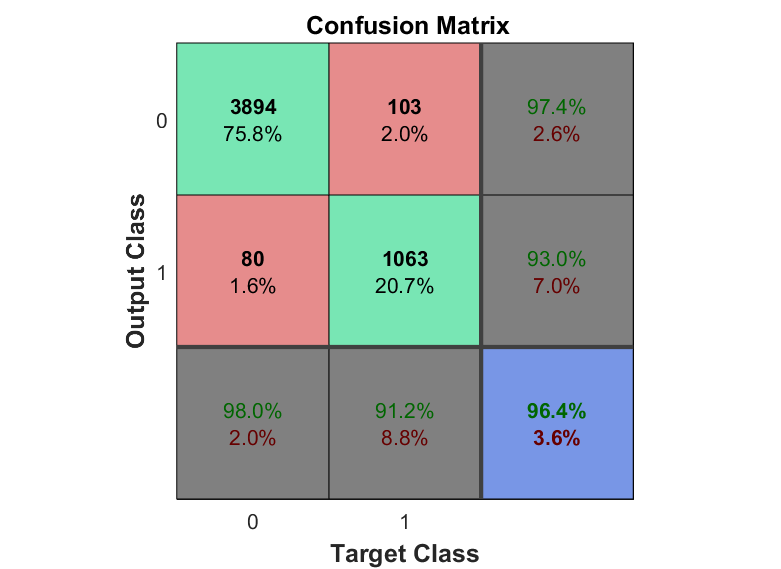
\includegraphics[width=\textwidth]{../figures/final/confmat.png}
        \caption{Confusion matrix.}
        \label{fig:confmat}
    \end{subfigure}
    \hfill %add desired spacing between images, e. g. ~, \quad, \qquad, \hfill etc. 
      %(or a blank line to force the subfigure onto a new line)
    \begin{subfigure}[t]{0.32\textwidth}
        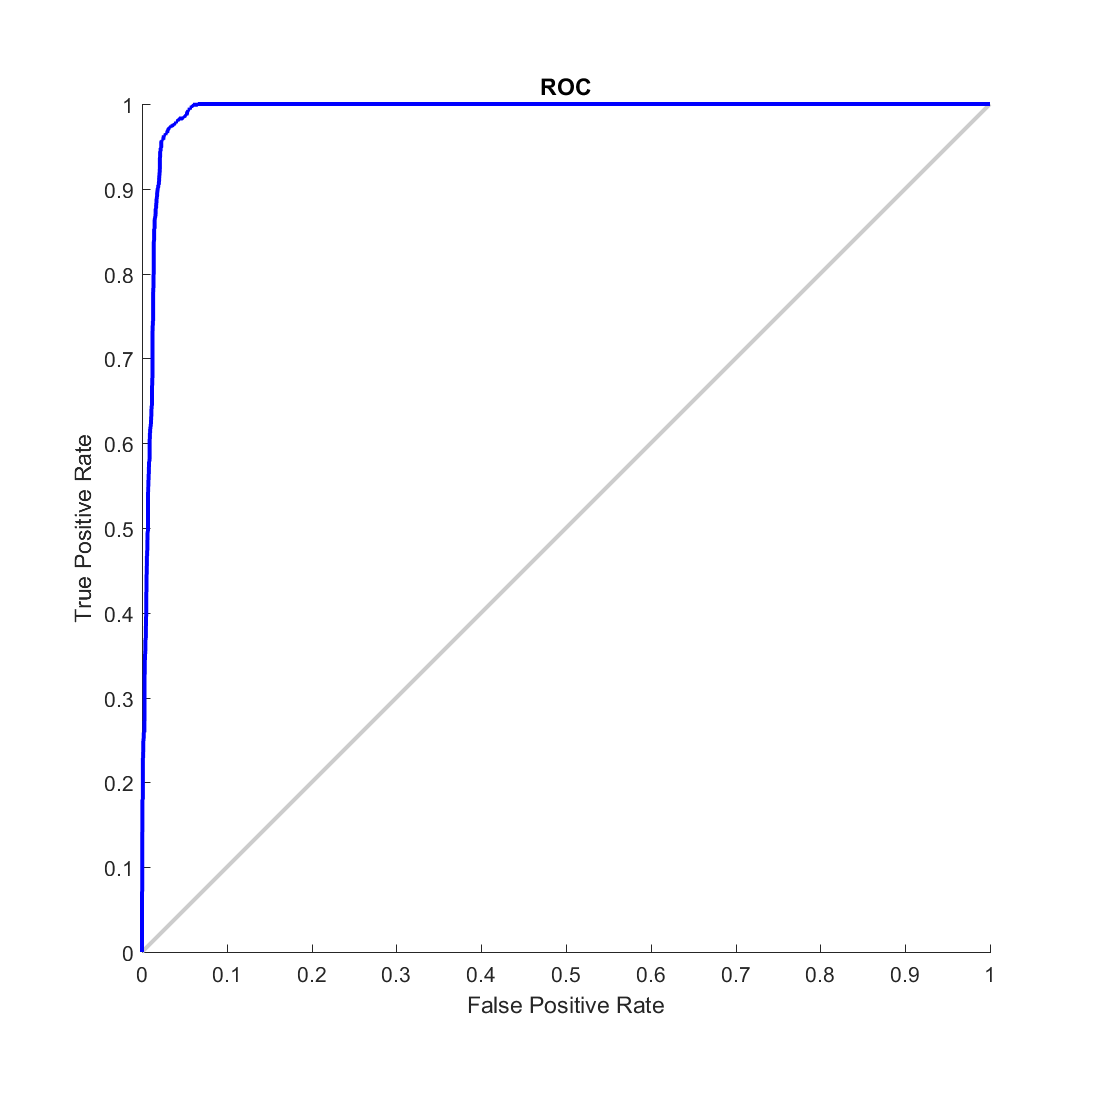
\includegraphics[width=\textwidth]{../figures/final/roc.png}
        \caption{ROC plot.}
        \label{fig:roc}
    \end{subfigure}
    \hfill %add desired spacing between images, e. g. ~, \quad, \qquad, \hfill etc. 
    %(or a blank line to force the subfigure onto a new line)
    \begin{subfigure}[t]{0.32\textwidth}
        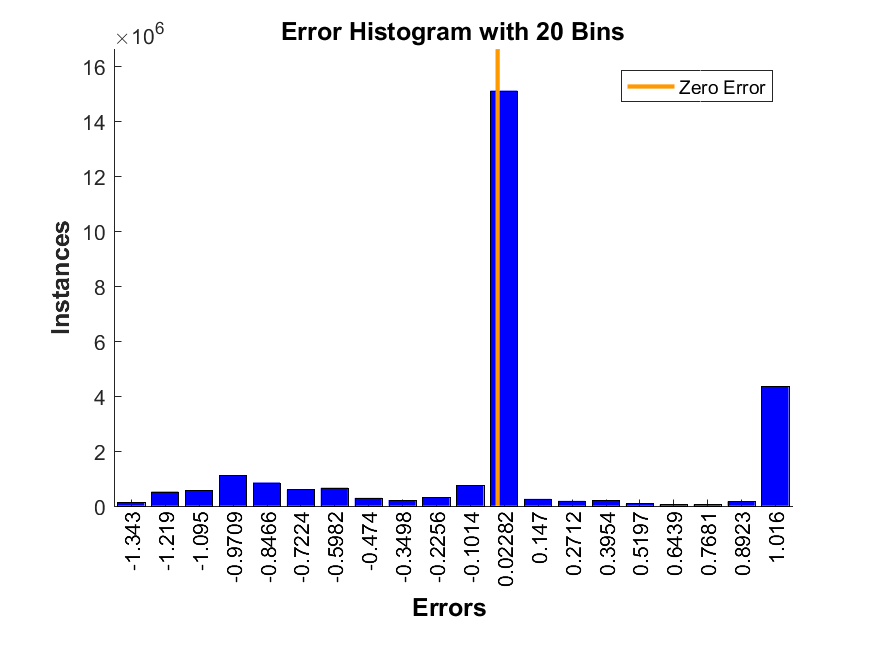
\includegraphics[width=\textwidth]{../figures/final/errhist.png}
        \caption{Error histogram.}
        \label{fig:errhist}
    \end{subfigure}
    \caption{Performance of RBFN with parameters $m = 20$ and $\epsilon = 0.6,0.7, 0.8, 0.9, 1.0, 1.1, 1.2$, ran 10  times for each parameter combination.}\label{fig:Accuracy of selected architecture on the test set from a single run.}
\end{figure}

From the confusion matrix we see that the network achieves 96.4\% accuracy with a relativly equal distribution of errors in both classes. The ROC plot indicates a very good classifier as well. However on the error histogram we see that there are a lot of errors at the far right. This indicates that the network wasn't even close to classifying these data points correctly. These maybe points located near near a class boundary which are misclassified due to noise or outliers, which are not in range of any of the RBFs. 

We also notice that the network shows a relatively small MSE even with a very small hidden layer. This could mean that the data we have isn't representative of the problem.

Comparing the performance of the RBFN to that of the models proposed in \cite{Candanedo2016} we see that we get approximately the same accuracy as the models using the same input variables.


\part*{Section B}




\bibliographystyle{plain}
\bibliography{science}


\pagebreak
\appendix
\appendixpage


\lstset{language=Matlab,%
    %basicstyle=\color{red},
    breaklines=true,%
    morekeywords={matlab2tikz},
    keywordstyle=\color{blue},%
    morekeywords=[2]{1}, keywordstyle=[2]{\color{black}},
    identifierstyle=\color{black},%
    stringstyle=\color{mylilas},
    commentstyle=\color{mygreen},%
    showstringspaces=false,%without this there will be a symbol in the places where there is a space
    numbers=left,%
    numberstyle={\tiny \color{black}},% size of the numbers
    numbersep=9pt, % this defines how far the numbers are from the text
    frame = single,
    emph=[1]{for,end,break},emphstyle=[1]\color{red}, %some words to emphasise
    %emph=[2]{word1,word2}, emphstyle=[2]{style},    
}



\section*{Data import script}
\lstinputlisting[caption=getData.m, label = listing:data]{../getData.m}

\pagebreak

\section*{Network creation script}
\lstinputlisting[caption=RBFN.m, label = listing:rbfn]{../rbnet.m}

\pagebreak

\section*{Network experimentation script}
\lstinputlisting[caption=runRBFN.m, label = listing:runrbfn]{../rbnetsearch.m}

\pagebreak

\section*{Transformation settings}
\begin{table}[h]
\csvautotabular{../trans1.csv}
\caption{mapstd transformation settings}
\label{table:mapstd}
\end{table}

%\begin{table}[h]
%\csvautotabular[
%before reading = \begin{adjustbox}{max width=\columnwidth},
%after reading=\end{adjustbox},
%]{../trans2.csv}
%\caption{processpca transformation settings}
%\label{table:pca}
%\end{table}


% Please add the following required packages to your document preamble:
% \usepackage{graphicx}
\begin{table}[h]
\centering
\resizebox{\textwidth}{!}{%
\begin{tabular}{|l|lllll|llll|}
\hline
properties        & \multicolumn{5}{c|}{transform}                       & \multicolumn{4}{c|}{inverseTransform}     \\ \hline
name = processpca & -0.37955 & -0.39547 & -0.40712 & -0.49929 & -0.53339 & -0.37955 & 0.52236  & 0.21998  & -0.69077 \\
xrows = 5         & 0.52236  & -0.58823 & 0.4643   & 0.10901  & -0.392   & -0.39547 & -0.58823 & 0.1784   & 0.065158 \\
maxfrac = 0.02    & 0.21998  & 0.1784   & 0.37132  & -0.85446 & 0.22761  & -0.40712 & 0.4643   & 0.37132  & 0.6934   \\
yrows = 4         & -0.69077 & 0.065158 & 0.6934   & 0.091391 & -0.17156 & -0.49929 & 0.10901  & -0.85446 & 0.091391 \\
nochange = 0      &          &          &          &          &          & -0.53339 & -0.392   & 0.22761  & -0.17156 \\ \hline
\end{tabular}%
}
\caption{processpca transformation settings}
\label{table:pca}
\end{table}


\end{document}
